\graphicspath{{chapters/03/images/}}
\chapter{Semi-empirical force fields}

\section{Introduction}
A protein system can be modelled using a force field, a description of the interactions between elements in the system.
A simulation needs a topology file which describes all of the interactions, the connecting information between atoms and the kind of force field that will be used.
To model protein systems semi-empirical force field are used.
The formula used in these kind of force fields are not rigorous: all the results from a simulation need to be validated through an experiment.

	\subsection{Potential energy surface}
	The state of any system can be described through a potential energy surface.
	The minima of the potential energy surface represents states in which the system will spend most of its time.
	The equilibrium state is found in the global minima of the surface.
	Lots of local minima are usually found on the surface and the system will jump between them during a simulation, with a frequency that depends on the deepness of the minima and the temperature of the environment.
	Statistical mechanics is necessary to compute the potential energy and the free energy surfaces at finite temperature, or when the jumping frequency is not zero.

		\subsubsection{Entropy}
		When dealing with these kind of computations entropy needs to be taken into account.
		To do so the conformational space, or the phase space, of the system needs to be explored so that compatible conformations for a certain condition can be found.

	\subsection{Types of force fields}
	Force fields can be categorized as:

	\begin{multicols}{2}
		\begin{itemize}
			\item All atoms: one atom corresponds to one bead.
			\item More atoms: more atoms correspond to one bead.
			\item Corse grained: groups of atoms correspond to one bead.
			\item Polarizzarle force fields: point charges are variables.
		\end{itemize}
	\end{multicols}

	As a golden rule parameters from different force fields should never be mixed.


\section{Computing the potential energy between bonded atoms}
When computing the potential energy of an atom its interactions with the other with which it forms a chemical bond needs to be considered.
The chemical bond can assume different conformations, each with a different value of potential energy.
Because the objective is to consider conformational transitions, the system will be completely modelled using classical mechanics, so bonds are unbreakable.
The potential energy surface used to describe an unbreakable bond can be seen in figure \ref{fig:chem-bond}.

\begin{figure}[H]
	\centering
	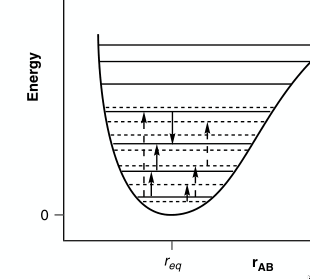
\includegraphics[width=0.5\textwidth]{chem-bond}
	\caption{Typical potential energy of a chemical bond}
	\label{fig:chem-bond}
\end{figure}

	\subsection{Bond stretching}
	During bond stretching the distance of two bonded atoms changes.
	To model this process consider the typical potential energy for a chemical bond in figure \ref{fig:chem-bond}.
	Let $r_{eq}$ the distance for which the energy is minimal, or where the equilibrium is.
	Moving from it the energy increases.
	When close to the minimum the well can be assumed symmetric.
	Asymmetry arises far from the minimum: it can be seen how the left part is steeper.
	Using a Taylor expansion the potential energy is approximated at point $r$ by taking the value at the equilibrium and then constructing all the corrections:

	$$U(r)=U(r_{eq}) + \frac{dU}{dr}\biggr\vert_{r=r_{eq}}(r-r_{eq})+\frac{1}{2!}\frac{d^2U}{dr^2}\biggr\vert_{r=r_{eq}}(r-r_{eq})^2+\frac{1}{3!}\frac{d^3U}{dr^3}\biggr\vert_{r=r_{eq}}(r-r_{eq})^3+\cdots$$

	Considering this expansion:

	\begin{multicols}{2}
	  \begin{itemize}
	    \item The first term is the value at equilibrium multiplied by the distance.
			\item The second term is the correction for the second derivative and so on.
	  \end{itemize}
	\end{multicols}

	Now a number of assumptions can be made:

	\begin{multicols}{2}
	  \begin{itemize}
	    \item If the potential is symmetric the first term is $0$ as it happens near the equilibrium.
				This makes the first term negligible.
			\item If the minimum is shallow the third term is $0$ and happens near the equilibrium.
				This makes the third term negligible.
	  \end{itemize}
	\end{multicols}

	\begin{align*}
		U(r)&=U(r_{eq}) + \xcancel{\frac{dU}{dr}\biggr\vert_{r=r_{eq}}(r-r_{eq}})+\frac{1}{2!}\frac{d^2U}{dr^2}\biggr\vert_{r=r_{eq}}(r-r_{eq})^2+\xcancel{\frac{1}{3!}\frac{d^3U}{dr^3}\biggr\vert_{r=r_{eq}}(r-r_{eq})^3}+\cdots\\
	\end{align*}

	So that in the end the typical harmonic potential is obtained:

	$$U(r_{AB}) = \frac{1}{2}k_{AB}(r_{AB}-r_{AB,eq})^2$$

	Considering that:

	\begin{multicols}{2}
	  \begin{itemize}
			\item $k$ is related to $\frac{d^2 U}{dr^2}$.
			\item The distances and $k$ are unique for each couple of atoms.
				An important issue for these parameters is transferability: these type of parameters need to be computed for each type of force field.
	  \end{itemize}
	\end{multicols}

		\subsubsection{Anharmonic force constant}
		Considering that the shape is not completely symmetric the third order term can be re-inserted in the formula when necessary.
		This introduces an asymmetry in the system, or an anharmonic force constant:

		$$U(r_{AB}) = \frac{1}{2}[k_{AB}+k^{(3)}_{AB}(r_{AB}-r_{AB, eq})](r_{AB}-r_{AB, eq})^2$$

		\subsubsection{Quartic correction}
		Also the fourth order term can be inserted for better accuracy:

		$$U(r_{AB}) = \frac{1}{2}[k_{AB}+k^{(3)}_{AB}(r_{AB}-r_{AB, eq}) + k^{(4)}_{AB}(r_{AB}-r_{AB,eq})^2](r_{AB}-r_{AB, eq})^2$$

		\subsubsection{Morse potential}
		The Morse potential is used in implicit solvent simulation.
		The exponential allows to describe screen interactions that happen with the implicit solvent.
		This is more difficult to compute, but it is also useful for soft or coarse-grained systems.

		$$U(r_{AB}) = D_{AB}\left[1-e^{-\alpha_{AB}(r_{AB}-r_{AB,eq})^2}\right]$$

	\subsection{Valence angle bending}
	When an atom makes multiple bonds with different atom the angle between the bonds can fluctuate around an equilibrium value.
	These events are described as valence angle bending.
	A valence angle is represented in \ref{fig:valence-angle-bending}.

	\begin{figure}[H]
		\centering
		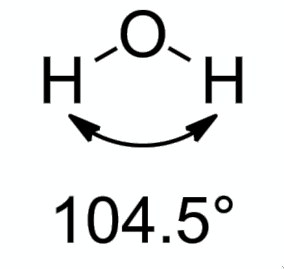
\includegraphics[width=0.3\textwidth]{valence-angle-bending}
		\caption{A valence angle}
		\label{fig:valence-angle-bending}
	\end{figure}

	In order to describe valence angle bending a Taylor expansion introducing an equilibrium angle is built.
	The first order term is not considered as it will be equal to $0$.
	Then the second introduces the harmonic potenital and the third for the anharmonic one, in principle also the quartic correction could be added.
	This formula is similar to the previous one but all the constant have to be described between each triplet of atoms:

	$$U(\theta_{ABC}) = \frac{1}{2}[k_{ABC}+k^{(3)}_{ABC}(\theta_{ABC}-\theta_{ABC,eq})+k^{(4)}_{ABC}(\theta_{ABC}-\theta_{ABC,eq})^2+\cdots](\theta_{ABC}-\theta_{ABC, eq})^2$$

		\subsubsection{Multiple minima}
		Another thing to consider when studying valence angle bending is that angles do not vary continuously: they wrap around at $\pi$ and $0$.
		This introduces a problem as the Taylor expansion cannot account for this event.

			\paragraph{Fourier expansion}
			To solve this problem the potential energy can be modelled thought a Fourier expansion.
			This operation introduces a periodic function that contains oscillations around a period, allowing to model any possible periodic potential, as the one for angles.

			\paragraph{Valence angle bending with a Fourier expansion}
			To parametrize the valence angle bending interaction a Fourier term is introduced, such that the terms are labelled with $j$.
			The amplitude, which multiplies each Fourier component decreases with $j$ and a cut-off on it is given, so to consider only low-frequency components.
			Now the potential energy for a valence angle bending interaction can be described by:

			$$U(\theta_{ABC}) = \sum\limits_{\{j\}_{ABC}}k^{fourier}_{j,ABC}[1+\cos(j\theta_{ABC}+\psi_j)]$$

			Where:

			\begin{multicols}{2}
			  \begin{itemize}
			    \item $\psi_j$ is the phase angle.
					\item The amplitude is computed as:

						$$k_{j, ABC}^{fourier} = \frac{2k^{harmonic}_{ABC}}{j^2}$$

			  \end{itemize}
			\end{multicols}

	\subsection{Torsions}
	Let $A, B, C$ and $D$ be $4$ atoms, bound according to $A->B->C->D$, like in figure \ref{fig:torsions}.
	Torsions describe the relative rotations of atoms $A$ and $D$ around the bond between $C$ and $D$.

	\begin{figure}[H]
		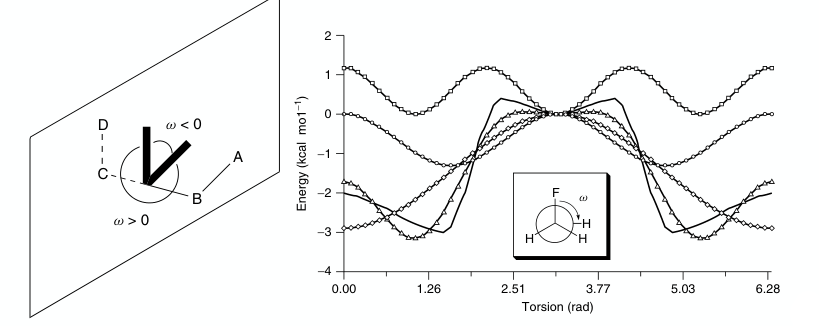
\includegraphics[width=\textwidth]{torsions}
		\caption{An example of torsion}
		\label{fig:torsions}
	\end{figure}

	To model this movement the planes $ABC$ and $BCD$ are built and the angle $\omega$ between them is considered.
	$\omega$ will describe the torsion around the bond.
	The angle is computed as the angle between the vectors perpendicular to the planes.
	The potential is computed through a Fourier expansion because it is periodic:

	$$U(\omega_{ABCD}) = \frac{1}{2}\sum\limits_{\{j\}_{ABCD}}V_{j,ABCD}\left[1+(-1)^{j+1}\cos(j\omega_{ABCD}+\psi_{j,ABCD})\right]$$

	All the possible groups of $4$ atoms, considering permutations and repetitions need to be parametrized to describe this potential.

		\subsubsection{Improper torsions}
		Improper torsions are a particular type of torsion that happens when the four atoms $A, B, C$ and $D$ are bound according to $A->B->C$ and $B->D$, like in figure \ref{fig:improper-torsions}.

		\begin{figure}[H]
			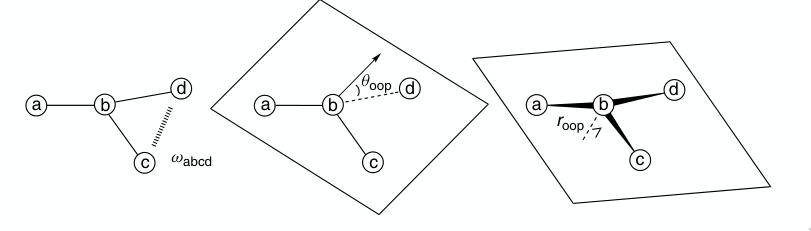
\includegraphics[width=\textwidth]{improper-torsions}
			\caption{An example of improper torsion}
			\label{fig:improper-torsions}
		\end{figure}

		$B$ can be in the same plane of $A, C, D$ or it can pop out.
		In this case two planes are built, usually $ABC$ and $BCD$ and the angle $\omega$ between them is considered.
		The potential will describe the energy of the angle.
		The angle can be computed as the out of plane angle $OOP$, obtaining the equation for the plane $ACD$ and computing how much $B$ is out of that plane.
		The potential is again described through a Fourier expansion:

		$$U(\omega_{ABCD}) = \frac{1}{2}\sum\limits_{\{j\}_{ABCD}}V_{j,ABCD}[1+(-1)^{j+1}\cos(j\omega_{ABCD}+\psi_{j,ABCD})]$$

		To parameterize this potential all possible groups of an atom connected with $3$ others need to be considered.
		The $sp^2$ hybridization constraints all the atoms in a plane.

\section{Non bonded interactions}

	\subsection{Van der Waals interactions}
	Van der Waals interactions happen whenever two atoms come close to one another without any chemical bond connecting them.
	It is a dispersion interaction and depends on the correlation of the electron clouds.
	This happens even if the electrons are not shared between atoms and depend only on the distance between them.
	The potential energy of a Van der Waals interaction is visualized in figure \ref{fig:van-der-waals}.
	Van der Waals interactions are a type of attractive forces that decrease with the $6$th power of the distance and it is closely related to a repulsion.
	The repulsion is due to Pauli's exclusion principle: whenever two atoms come close an energy level becomes occupied and it stops them to become closer.
	This is difficult to compute, so it is modelled through an hard limit, modelled by the $12$th power of the distance, making the energy become very high whenever the distance becomes less than the equilibrium.

	\begin{figure}[H]
		\centering
		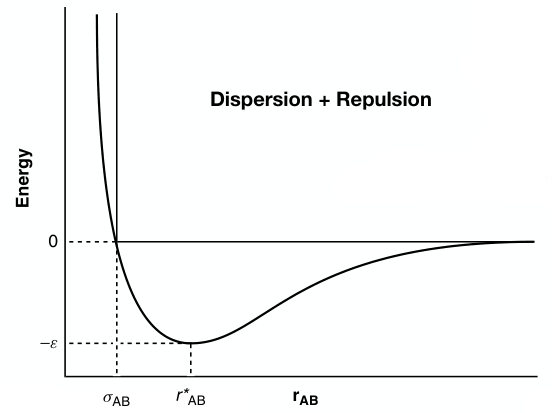
\includegraphics[width=0.5\textwidth]{van-der-waals}
		\caption{Energy of a Van der Waals interaction}
		\label{fig:van-der-waals}
	\end{figure}

		\subsubsection{Lennard-Jones potential}
		The Lennard-Jones potential models both the attraction due to the Van der Waals interaction and the repulsion due to Pauli's exclusion principle.
		The corresponding formula is cheap to compute but has no physical basis:

		\begin{align*}
			U_(r_{AB}) &= \frac{a_{AB}}{r^{12}_{AB}}-\frac{b_{AB}}{r^6_{AB}}=\\
								 &= 4\epsilon_{AB}\biggl[\biggl(\frac{\sigma_{AB}}{r_{AB}}\biggr)^{12}-\biggl(\frac{\sigma_{AB}}{r_{AB}}\biggr)^6\biggr]
		\end{align*}

		And the distance with minimum energy or equilibrium is:

		$$r^*_{AB} = 2^{\frac{1}{6}}\sigma_{AB}$$

		Where $\sigma_{AB}$ is the Van der Waals radius, where the energy is $-\epsilon$.
		A value of $\sigma_{AB}$ have to be introduced for any couple of types of atoms.

		\subsubsection{Morse potential}
		The Morse potential is usually used with coarse grained systems or with soft-matter simulations.
		This potential has the same features of the Lennard-Jones potential:

		$$U(r_{AB}) = D_{AB}[1-e^{-a_{AB}(r_{AB}-r_{AB,eq})^2}]$$

		\subsubsection{Hill potential}
		The Hill potential is usually used with coarse grained systems or with soft-matter simulations.
		This potential has the same features of the Lennard-Jones potential:

		$$U(r_{AB}) = \epsilon_{AB}\biggl[\frac{6}{\beta_{AB}-6}e^{\beta_{AB}\frac{1-r_{AB}}{r^*_{AB}}}-\frac{\beta_{AB}}{\beta_{AB}-6}\biggl(\frac{r^*_{AB}}{r_{AB}}\biggr)^6\biggr]$$

		\subsubsection{Scaling for already accounted interactions}
		In some force fields $1$-$4$ interactions are reduced by a scaled factor, while in other are completely removed.
		This is because in these force fields the torsions are modelled such that they already take into account these proximity effects.

	\subsection{Electrostatic interactions}
	Electrostatic interactions happen between charged or polar molecules.
	To model these kind of interactions the distribution of charges needs to be described.
	In principle a multiple expansion should be performed.
	The shape of the clouds of charges should be given for each molecules and each interaction should be described by the matrix multiplication of all the matrices:

	$$U_{AB} = \vec{M}^{(A)}V^{(B)}$$

	Now, summing over all molecules:

	$$U_{AB} = \sum\limits_{A}\sum\limits_{B>A}\vec{M}^{(A)}\vec{V}^{(B)}$$

	This is a very costly procedure but provides accurate results.

		\subsubsection{Point like charges}
		To make the computation easier molecules are represented as point-like partial charges.
		Each atom in a molecule is assumed to be point like and to have a partial charge.
		The electron cloud is displaced toward the negative cloud and away from the positive one.
		In this way the distribution of charges can be represented by numbers placed on each atom.
		Once this is done an electric charge is associated with each bead and the Coulomb interaction is used to compute the energy:

		$$U_{AB} = \frac{q_Aq_B}{\epsilon_{AB}r_{AB}}$$

		Where $\epsilon_{AB}$ is the dielectric constant and depends on the type of solvent ($1$ for explicit ones).

		\subsubsection{Dipolar interactions}
		Dipolar interaction can be included when considering electrostatic forces.
		These formulae are mostly used in corse grained models: approximation of single charges one a bead cannot be made.
		The interaction takes a functional form with a number of parameters:

		Because in that case the approximation of single charges on a bead cannot be made and dipoles are considered.
		In this case a functional form and the parameters need to be included.
		The energy is computed as:

		$$U_{AB/CD} = \frac{\mu_{AB}\mu_{CD}}{\epsilon_{AB/CD}r^3_{AB/CD}}(\cos\chi_{AB/CD}-3\cos\alpha_{AB}\cos\alpha_{CD})$$

		Where:

		\begin{multicols}{2}
		  \begin{itemize}
		    \item $\mu$ is the dipole of two molecules.
				\item $\epsilon_{AB/CD}$ is the dielectric constant.
				\item The cosine term represents the orientation of the two dipoles.
		  \end{itemize}
		\end{multicols}

		\begin{figure}[H]
			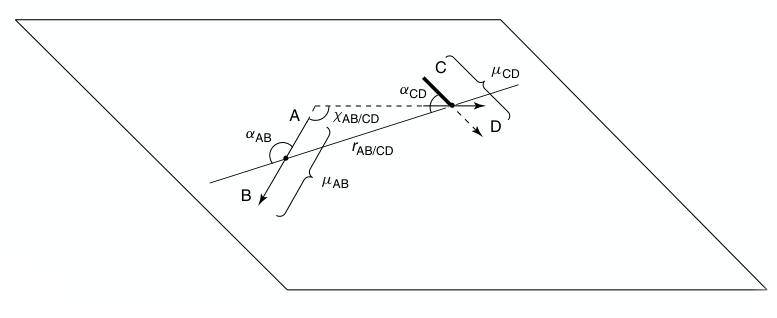
\includegraphics[width=\textwidth]{dipolar-interactions}
			\caption{An example of a dipolar interaction}
			\label{fig:dipolar-interactions}
		\end{figure}

		\subsubsection{Dielectric constants}
		The dielectric constant changes depending on the type of interaction the atom.
		For example:

		$$\epsilon_{AB} = \begin{cases}\infty&\text{ if }A\land B\text{ are 1,2- or 1,3-related}\\3.0&\text{ if }A\land B\text{ are 1,4-related}\\1.5&\text{otherwise}\end{cases}$$

		These scaling factors depend on the force field chosen.

\section{Cross terms}
Different type of interactions depend between each other, so all the possible degree of freedom should be considered together:

\begin{align*}
	U(\vec{q}) = &U(\vec{q}_{eq}) + \sum\limits_{i=1}^{3N-6}(q_i-q_{i,eq})\frac{\partial U}{\partial q_i}\biggr\vert_{\vec{q}=\vec{q}_{eq}} + \\
							 &+\frac{1}{2!}\sum\limits_{i=1}^{3N-6}\sum\limits_{j=1}^{3N-6}(q_i-q_{i,eq})(q_j-q_{j,eq})\frac{\partial^2 U}{\partial q_i\partial q_j}\biggr\vert_{\vec{q}=\vec{q}_{eq}} +\\
							 &=\frac{1}{3!}\sum\limits_{i=1}^{3N-6}\sum\limits_{j=1}^{3N-6}\sum\limits_{k=1}^{3N-6}(q_i-q_{i,eq})(q_j-q_{j.eq})(q_k-q_{k,eq})\frac{\partial^3 U}{\partial q_i\partial q_j\partial q_k}\biggr\vert_{\vec{q}=\vec{q}_{eq}} + \cdots
\end{align*}

This is done by starting from a Lagrangian describing all the interaction and compute all the terms.
In practice, besides some force fields, everything is done without considering them:

$$U(r_{AB}, \theta_{ABC}) = \frac{1}{2}k_{AB,ACB}(r_{AB}-r_{AB, eq})(\theta_{ABC}-\theta_{ABC, eq})$$

\section{Parametrization}
All the interactions need a large set of parameters to be computed, which grows with the number of atoms $N$ as:

$$p = N + (N-1)+(N-2)+\cdots = N\frac{N+1}{2}$$


	\subsection{Obtaining the parameters}
	The parameters are obtained comparing experimental data (from which the term semi-empirical) with the results of a simulation.
	Then the penalty function is introduced:

	$$Z = \biggl[\sum\limits_{i}^{observables}\sum\limits_{j}^{occurrences}\frac{(calc_{i,j}-expt_{i,j})^2}{w_i^2}\biggr]^{\frac{1}{2}}$$

	This is summed over all the data from all the observables.
	Then it is minimized by changing the simulation's parameters until a reasonable compromise is reached.
	This is the reason for the constant update of the force fields.

	\subsection{Reducing the number of parameters}
	To reduce the number of parameters, they are factorized so that they need to be defined only for each atom:

	\begin{align*}
		\sigma_{AB} &= \sigma_A+\sigma_B\\
		\epsilon_{AB} &= (\epsilon_A\epsilon_B)^{\frac{1}{2}}
	\end{align*}

	\subsection{Geometry optimization}
	It may happen that two atoms are too close to each other at the start of a simulation, leading to high forces, kicking out the atom and causing the simulation to explode.
	Geometry optimization is done to obtain the parameters or to minimize them so to avoid high forces values at the start of a simulation.
	To do so the gradient of the energy is computed and the system is moved toward the minimum energy.
	The derivative need to be computed of $U$ with respect to each component in the system.

	$$\vec{g}(\vec{q}) = \begin{bmatrix} \frac{\partial U}{\partial q_1} \\ \frac{\partial U}{\partial q_2} \\ \vdots \\ \frac{\partial U}{\partial q_n}\end{bmatrix}$$

	Such that the cost reaches the global minimum $J_{min}(\vec{w})$.

		\subsubsection{Derivative of the potential function}
		First the derivatives need to be computed.
		All the potentials are given in term of the mutual distance of two atoms.
		So, considering $x$ the coordinates of a point:

		$$\frac{\partial U}{\partial x_A} = \sum\limits_{i\in A}\frac{\partial U}{\partial r_{Ai}}\frac{\partial r_{Ai}}{\partial x_A}$$

		Taking the derivative of this:

		$$U(r_{AB}) = \frac{1}{2}[k_{AB}+k_{AB}^{(3)}(r_{AB}-r_{AB, eq}) + k_{AB}^{(4)}(r_{AB}-r_{AB, eq})^2](r_{AB}-r_{AB,eq})^2$$

		With respect to the distance:

		$$\frac{\partial U}{\partial r_{Ai}} = \frac{1}{2}[2k_{Ai}+3k_{Ai}^{(3)}(r_{Ai}-r_{Ai, eq}) + 4k^{(4)}_{Ai}(r_{Ai}-r_{Ai, eq})^2](r_{Ai}-r_{Ai, eq})$$

		In order to take the derivative with respect to $r$ the derivative with to $x$ needs to be known:

		$$\frac{\partial r_{Ai}}{\partial x_A} = \frac{x_A-x_i}{\sqrt{(x_A-x_i)^2+(y_A-y_i)^2+(z_A-z_i)^2}}$$

		Then this formula can plugged in according to the chain rule.

		\subsubsection{Newton-Raphson}
		The minimization for geometry optimization is performed as an iterative procedure: the Newton-Raphson.
		Consider $(n)$ as the identifier for the $n$th iteration.
		This allow to obtain iteration $k+1$ via a Taylor expansion of coordinates at iteration $k$:

		$$U(\vec{q}^{(k+1)}) = U(\vec{q}^{(k)}) + (\vec{q}^{(k+1)} -\vec{q}^{(k)})\vec{g}^{(k)} + \frac{1}{2}(\vec{q}^{(k+1)}-\vec{q}^{(k)})H^{(k)}(\vec{q}^{(k+1)}-\vec{q}^{(k)})$$

		Where $H$ is the Hessian matrix:

		$$H_{ij}^{(k)} = \frac{\partial^2 U}{\partial q_i\partial q_j}\biggr\vert_{\vec{q}=\vec{q}^{(k)}}$$

		And:

		$$\frac{\partial U(\vec{q}^{(k+1)})}{\partial q_i^{(k+1)}} = \frac{\partial \vec{q}^{(k+1)}}{\partial q_i^{(k+1)}}\vec{g}^{(k)}+ \frac{1}{2}\frac{\partial \vec{q}^{(k+1)}}{\partial q_i^{(k+1)}}H^{(k)}(\vec{q}^{(k+1)}-\vec{q}^{(k)})+\frac{1}{2}(\vec{q}^{(k+1)}-\vec{q}^{(k)})H^{(k)}\frac{\partial \vec{q}^{(k+1)}}{\partial q_i^{(k+1)}}$$

		So that:

		$$\vec{g}_i^{(k+1)} = \vec{g}_i^{(k)} + [H^{(k)}(\vec{q}^{(k+1)}-\vec{q}^{(k)})]_i$$

		After enough iterations the system reaches a stationary conditions, where the system won't change in successive iterations:

		$$\vec{0} = \vec{g}^{(k)} + H^{(k)}(\vec{q}^{(k+1)}-\vec{q}^{(k)})\Rightarrow \vec{q}^{(k+1)} = \vec{q}^{(k)} - [H^{(k)}]^{-1}\vec{g}^{(k)}$$
